\section{Processing time per visit}
\label{sec:visit_timing}
A visit is one block of the campaign: an arc, a lamp flat and the exposures of the target (2 for Fairall~9).
Table~\ref{tab:visit_timing} breaks the processing time of each frame type into the pipeline stages, measured
from the time stamps of the \banzai{} log for the final configuration (one worker; four ran in parallel on an
8-core laptop with 8\,GB of memory). Figure~\ref{fig:visit_timing} adds them up per visit.

\begin{table}[!htbp]
\centering
\caption{Median processing time per frame (s, one worker) by pipeline stage, final configuration. ``Arc'' is
the 2-d wavelength solution; ``orders'' the order loading and tweak; ``fringe'' the lamp-pattern loading and the
harmonic fit (joint with the telluric template); ``flux + telluric'' the sensitivity, the ensemble flux
calibration and the telluric correction; ``other'' reading, writing and database access.}
\label{tab:visit_timing}
\small
\begin{tabular}{lcccccccccc}
\toprule
Frame & $N$ & arc & orders & fringe & trace & bkg+CR & extract & flux+tell & other & total \\
 & (frames) & (s) & (s) & (s) & (s) & (s) & (s) & (s) & (s) & (s) \\
\midrule
Arc & 122 & 46.3 & 0.2 & -- & -- & -- & 1.2 & -- & -- & 48 \\
Lamp flat & 133 & 0.7 & 0.4 & -- & -- & -- & 0.5 & -- & 2.4 & 4 \\
Standard & 39 & 0.5 & 0.3 & 0.9 & 5.4 & 1.9 & 1.5 & 0.8 & -- & 12 \\
Science & 118 & 0.5 & 0.3 & 0.9 & 3.5 & 1.8 & 2.0 & 0.3 & 0.1 & 10 \\
\bottomrule
\end{tabular}
\end{table}

\begin{figure}[!htbp]
\centering
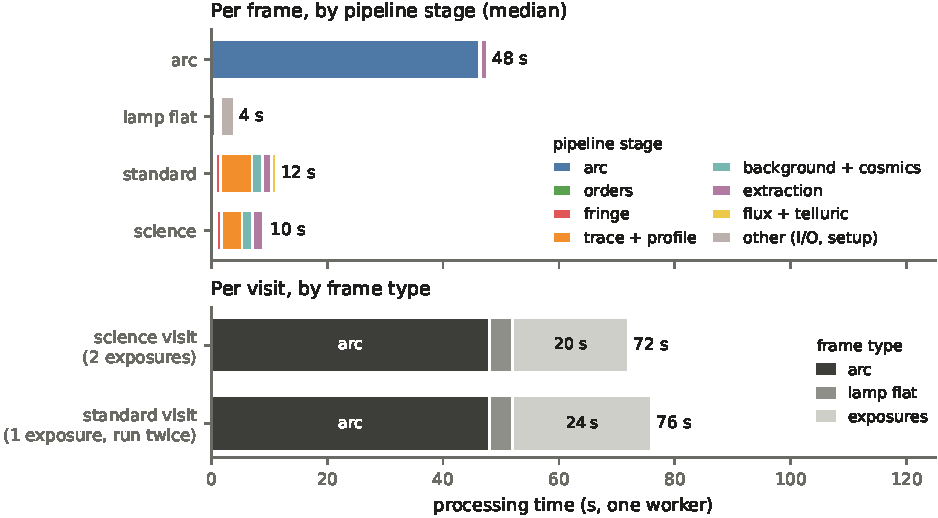
\includegraphics[width=\textwidth]{figures/fig_visit_timing.pdf}
\caption{Left: median processing time per frame by stage. Right: per visit, for a science visit (arc, lamp flat
and 2 exposures) and a standard visit (arc, lamp flat and one exposure, processed twice: before and after the
residual fringe template is measured).}
\label{fig:visit_timing}
\end{figure}

A science visit costs $\approx72$\,s of processing (48\,s arc, 4\,s lamp flat,
2$\times$10\,s for the exposures) and a standard visit $\approx76$\,s. With four workers
the throughput is $\approx18$\,s of wall-clock time per science visit, so the
$\approx5000$ visits of a decade take $\approx25$\,h on this laptop, most of it in the arcs.
Fitting the arc once per instrument epoch and checking each block only for a zero-point shift
(Chapter~\ref{sec:wavelength}) would bring this to $\approx8$\,h. The steps that are not
per frame are small: the fringe phase master of a slit and two-month window takes 3\,s,
the residual fringe template 3\,s, and the ensemble flux and telluric calibrations
read the nearest nine standards from the database for each frame (included in ``flux + telluric'').
